\section{The field equations of gravity}

\begin{frame}{Sliiiiiding}
    The field equations of gravity are \cite{Einstein:1915ca}
    \begin{equation}
        R_{\mu\nu}-\frac{1}{2}g_{\mu\nu}R + \Lambda g_{\mu\nu}= \frac{8\pi \symup{G}}{\symup{c}^4} T_{\mu\nu}.
    \end{equation}

    \subsection{Solutions}
    The \emph{Schwarzschild} solution is:
    \begin{equation}
        \dif s^2 = \l( 1 - \frac{r_{\symup{s}}}{r} \r) \symup{c}^2 \,\dif t^2 - \l(1-\frac{r_{\symup{s}}}{r}\r)^{-1} \,\dif r^2 - r^2 \l(\dif \Theta^2+\sin^2\Theta \dif \varphi^2\r).
    \end{equation}
    This is a vacuum solution ($T_{\mu\nu}=0$) \footnotemark[1]
    \footnotetext[1]{\fullcite{Einstein:1915ca}}
\end{frame}

\begin{frame}{On Footnotes}
    \begin{columns}[]
        \begin{column}{.5\textwidth}
            For citations directly on the page:\\
            First use \texttt{\small \backslash footnotemark[i]} \footnotemark[1]
        \end{column}
        \begin{column}{.5\linewidth}
            And then\\
            \texttt{\small \backslash footnotetext[i]\{\backslash fullcite\{citation\}\}}
        \end{column}
    \end{columns}

    \footnotetext[1]{So this is under \emph{all} columns}
\end{frame}

\section{On Quantizing Gravity}
\begin{frame}{Comprehensive Slide Title}
    HaHaHa. No.

    \begin{figure}
        \centering
        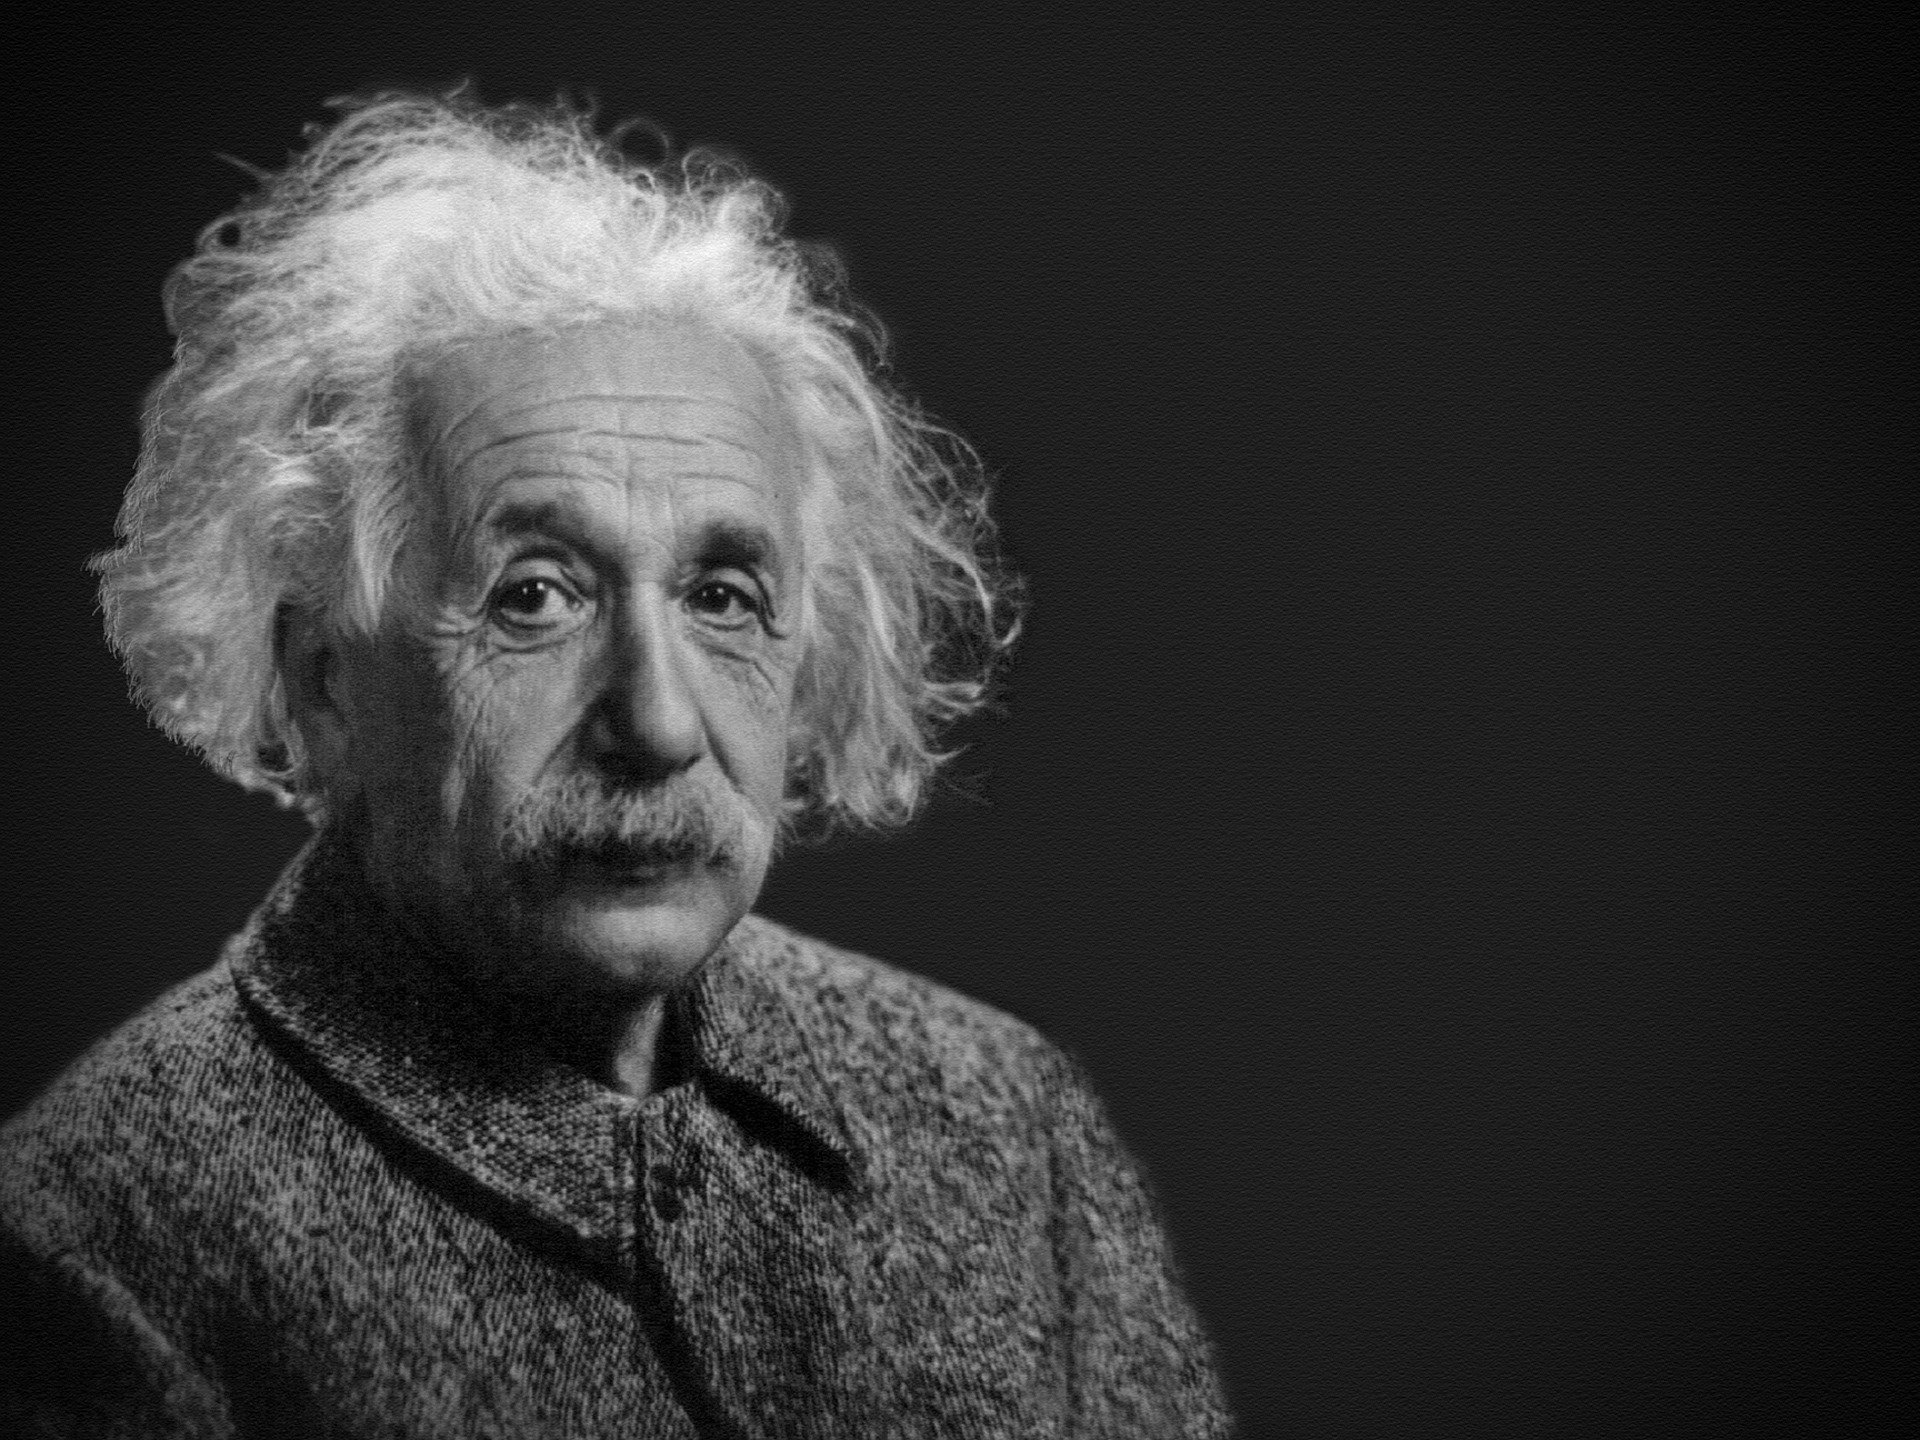
\includegraphics[width=0.3\textwidth]{media/einstein.jpg}
        \caption{Albert E. $=mc^2$}%
        \label{fig:einstein}
    \end{figure}
\end{frame}

